\chapter{Introduction} \label{ch:introduction}

This is a very short guide to an unofficial thesis/dissertation template for the University of Tennessee. It has been updated to meet the specifications as of 2023 but can be easily altered as the guidelines are changed. This template requires a basic knowledge of \LaTeX\ and should cover the basic requirements in terms of required packages and functionality.

\section{Disclaimer}
\textcolor{red}{\bf
This template is distributed AS IS WITH NO WARRANTY. It serves as a guideline and constitutes a basic structure for a thesis/dissertation. The user assumes full responsibility for formatting and typesetting their document and for verifying that all the thesis requirements set by the University of Tennessee are met. Please refer to the most recent UT thesis guide 
or contact the thesis consultant to whom you should also report bugs.}

\section{Getting started}
The general structure of this template is based on the tree shown in Figure \ref{fig:intro-folder-structure}. The titles of the folders are self descriptive and should guide you to proper file placement. Note that this is only a suggested model that could be modified to fit your own organizational structure.
You will find the mentioned figure on the next page. This is in accordance with Graduate School policy which states that so-called floats should not appear alongside with text. 

\begin{figure}[p]
  \centering
  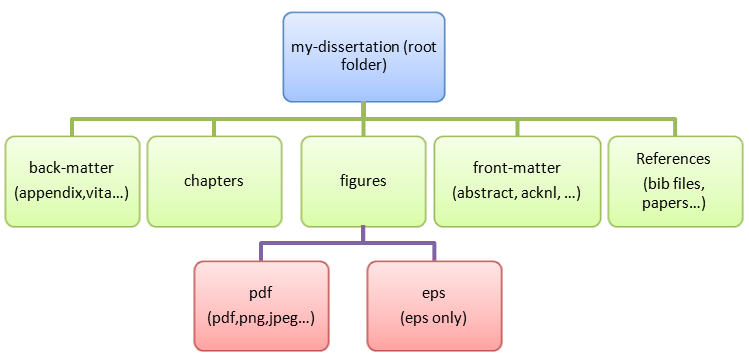
\includegraphics[width=6.5in]{fig01-folder-structure}\\
  \caption{UT thesis template folder structure.}\label{fig:intro-folder-structure}
\end{figure}

\subsection{Important Files}
There are two important files in this template: utthesis.cls and my-dissertation.tex.
\begin{itemize}

\item
utthesis.cls: Based on the report class, this file contains customized settings, definitions, packages, and macros. The file is located in the root directory. One or more of the packages included may conflict with a package that you want to add. If so, you must resolve the conflict either by removing the unused package or by modifying settings for either package. Preloaded packages include amsmath, amsthm, amssymb, setspace, geometry, hyperref, and color.

\item
my-dissertation.tex: This is the main file for your thesis/dissertation that brings everything together. Each individual section of your dissertation should be its own .tex file saved in the proper place. For example, a chapter for your dissertation should be saved in the chapters directory while your acknowledgments should be saved in the front-matter directory. You compile my-dissertation.tex to create a complete pdf that can be printed/shared. You may want to change the name of the file to my-name-dissertation.tex. The utthesis document class takes all the options for the report class in addition to thesis/dissertation and monochrome options. If you are writing a thesis, you must use "thesis" otherwise, use "dissertation" or omit that option because dissertation is the default setting. The monochrome option converts all your document to monochrome - except figures. This may be useful when printing your document since this dissertation has colored hyperlinks which tend to look washed out when printed on a monochrome printer. 
\end{itemize}


\subsection{Updating Information}
Your next step is to update information in my-dissertion.tex such as the document title, your name, degree, etc. 
This can be done as follows.

\begin{verbatim}
%%%%%%%%%%%%%%%%%%%%%%%%%%%%%%%%%%%%%%%%%%%%%%%%%%%%%%%%%%%%%%%%%%%%%
% TO DO: FILL IN YOUR INFORMATION BELOW - READ THIS SECTION CAREFULLY
%%%%%%%%%%%%%%%%%%%%%%%%%%%%%%%%%%%%%%%%%%%%%%%%%%%%%%%%%%%%%%%%%%%%%
\title{Thesis or Dissertation Title}	 % title 
\author{My Name}                         % your name
\copyrightYear{20XX}            		 % copyright year 
\graduationMonth{Month}           	     % month of graduation 
\degree{Degree}   % degree: Doctor of Philosophy, Master of ...
\university{The University  of Tennessee, Knoxville}	% school 
%%%%%%%%%%%%%%%%%%%%%%%%%%%%%%%%%%%%%%%%%%%%%%%%%%%%%%%%%%%%%%%%%%%%%
\end{verbatim}

\clearpage

\section{References}
The bibliography style used in this template is "apalike". It is an author-year style based on the APA specification. 
Here is example \citep{Fermi1956,Iznogood2000}. Many other bibliograhy style exist. See documentation elsewhere.
\begin{verbatim}
\bibliographystyle{apalike}
\bibliography{references-dissertation}
\end{verbatim} 
The second line specifies the .bib file that lists your references. Remember to run BibTeX in order to compile the bibliography. 

\section{Theorem environments}
This template contains predefined theorem, lemma, proposition, corollary, and definition environments. Numbering and other
style matters can be changed in the ``utthesis.clc'' file.

\begin{definition}
	This is an example of a definition.
\end{definition}
\begin{proposition}
	This is an example of a proposition.
\end{proposition}
\begin{theorem}[First theorem]\label{thm:theorem-a}
    This is an example theorem.
\end{theorem}
\begin{proof}[Proof for theorem]
    This is the proof for this theorem.
\end{proof}
\begin{lemma}[First lemma]
    This is the first lemma.
\end{lemma}
\begin{proof}
	This is the proof for this lemma that requires Theorem \ref{thm:theorem-a}.
\end{proof}
\begin{corollary}
    This is the first corollary.
\end{corollary}

\section{Figures and Tables}

\subsection{General Rules}
To comply with Graduate School formatting rules, 
figure captions should be placed below the figure and table captions should be placed above the table. Also, figures and tables should appear on pages of their own with no text (except for the caption of course). You must allow figures and table to float. DO NOT HARD CODE POSITIONS. In addition, no figure or table should spill into the margins. Should that happen, either resize it so that it or put it on its own landscape oriented page. See Figure \ref{fig:wide-pic} for an example of the latter. Note the page number location in the example. The code for this is given by:

\begin{verbatim}
\begin{landscape}
\begin{figure}[h]
    \centering
    \fbox{\rule{8in}{0pt}\rule{0pt}{5in}}
    \caption{This figure is too wide for a portrait page.}
    \label{fig:wide-pic}
\end{figure}
\end{landscape}
\end{verbatim}

Be careful about where you place this landscape page, as well as all figures and tables. These objects are not considered part of the text, and thus their placement should not be assigned to a precise location. The general rule to follow is that no text page should have significant white space, with the exception being the last page of a chapter. So if you mention a figure in some paragraph but the figure will not fit on the remainder of the page, continue the text (even if it's a new section) to fill the current page with text and then place the figure on the next page. 


\begin{landscape}
	\begin{figure}[p]
		\centering
	    \fbox{\rule{8in}{0pt}\rule{0pt}{5in}}
		\caption{This figure is too wide for a portrait page.}
		\label{fig:wide-pic}
	\end{figure}
\end{landscape}

\subsection{Single figures}

Single figures can created as shown below.
For more information, see \\ \href{http://en.wikibooks.org/wiki/LaTeX/Floats,_Figures_and_Captions}{http://en.wikibooks.org/wiki/LaTeX/Floats,\_Figures\_and\_Captions}.

\begin{verbatim}
    \begin{figure}[t for top, b for bottom, h for here, 
                   p for page with float(s) but no text]
        % Requires \usepackage{graphicx}
        \centering % center the figure
        \includegraphics[width=5in or 127mm etc...]{figure-name}\\
        \caption{figure caption}\label{figure label}
    \end{figure}
\end{verbatim}

\subsection{Multipart figures}

For multipart figures, use the package "subfig". You can
add space between the figures using spacing commands such as ``\verb|\qquad|''. For example, 

\begin{verbatim}
\begin{figure}[p]
   \centering
   \subfloat[Circle]{\label{fig:fig-a-space}
\includegraphics[width=1in]
     {fig02a-circle}} \qquad
   \subfloat[Rectangle]{\label{fig:fig-b-space}
\includegraphics[width=1in]
     {fig02b-rectangle}}\qquad
   \subfloat[Cube]{\label{fig:fig-c-space}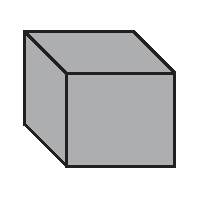
\includegraphics[width=1in]
     {fig02c-cube}}\qquad
   \caption{Geometric shapes with space between images.}
   \label{fig:multipart-figure-space}
\end{figure} 
\end{verbatim}

\begin{figure}[p]
  \centering
  
\includegraphics[width=1in]{fig02a-circle}\\
  \caption{Simple figure example.}\label{fig:simple_example}

  \vskip 20pt

  \subfloat[Circle]{\label{fig:fig-a-space}
\includegraphics[width=1in]{fig02a-circle}} \qquad
  \subfloat[Rectangle]{\label{fig:fig-b-space}
\includegraphics[width=1in]{fig02b-rectangle}}\qquad
  \subfloat[Cube]{\label{fig:fig-c-space}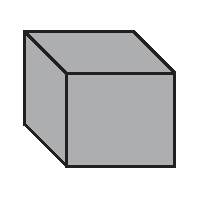
\includegraphics[width=1in]{fig02c-cube}}\qquad
  \caption{Example showing multiple subfigures.}
  \label{fig:multipart-figure-space}
\end{figure} 

\subsection{Tables}

Again, table captions should be placed above the table. See Table \ref{tab:table-a} for an example. 
For more information about tables, 
see \href{https://en.wikibooks.org/wiki/LaTeX/Tables}{https://en.wikibooks.org/wiki/LaTeX/Tables}.

Be aware that LaTeX may decide to group multiple floats together on the no-text page. 
If you don't like the resulting layout, try different placement options or move
one or more floats before or after a large body of text to break the flow. 
An alternative to the \verb+[p]+ option is 
\verb+\clearpage+ which flushes any remaining floats before continuing on a new page. 
The command \verb+\newpage+ breaks to a new page without flushing floats. 

\begin{table}[p]
\caption{A simple table with info on Smokey}
\label{tab:table-a}
\begin{center}
\begin{tabular}[b]{|c|c|c|c|}
	\hline
	Dog & Years & Record & Pct. \\ \hline
	Blue Smokey & 1953-1954 & 10-10-1 & .500 \\ \hline
	Smokey II & 1955-1963 & 58-39-5 & .597 \\ \hline
	Smokey III & 1964-1977 & 105-39-5 & .729 \\ \hline
	Smokey IV & 1978-1979 & 12-10-1 & .545 \\ \hline
	Smokey V & 1980-1983 & 28-18-1 & .608 \\ \hline
	Smokey VI & 1984-1991 & 67-23-6 & .744 \\ \hline
	Smokey VII & 1992-1994 & 27-9 & .750 \\ \hline
	Smokey VIII & 1995-2003 & 91-22 & .805 \\ \hline
	Smokey IX & 2004-2012 & 62-53 & .539 \\ \hline
	Smokey X & 2013-present & 21-17 & .552 \\ \hline
\end{tabular}
\end{center}
\end{table}


